%
% teil0.tex -- Definition
%
% (c) 2020 Prof Dr Andreas Müller, Hochschule Rapperswil
%
\section{Definition\label{fresnel:section:teil0}}
\rhead{Definition}
Die Funktion $e^{x^2}$ hat bekanntermassen keine elementare Stammfunktion,
weshalb die Fehlerfunktion als Stammfunktion definiert wurde.
Die Funktionen $\cos x^2$ und $\sin x^2$ sind eng mit $e^{x^2}$
verwandt, es ist daher nicht überraschend, dass sie ebenfalls
keine elementare Stammfunktionen haben.
Dies rechtfertigt die Definition der Fresnel-Integrale als neue spezielle
Funktionen.

\begin{definition}
Die Funktionen 
\begin{align*}
C(x) &= \int_0^x \cos\biggl(\frac{\pi}2 t^2\biggr)\,dt
\\
S(x) &= \int_0^x \sin\biggl(\frac{\pi}2 t^2\biggr)\,dt
\end{align*}
heissen die Fresnel-Integrale.
\end{definition}

Der Faktor $\frac{\pi}2$ ist einigermassen willkürlich, man könnte
daher noch allgemeiner die Funktionen
\begin{align*}
C_a(x) &= \int_0^x \cos(at^2)\,dt
\\
S_a(x) &= \int_0^x \sin(at^2)\,dt
\end{align*}
definieren, so dass die Funktionen $C(x)$ und $S(x)$ der Fall
$a=\frac{\pi}2$ werden, also
\[
\begin{aligned}
C(x) &= C_{\frac{\pi}2}(x),
&
S(x) &= S_{\frac{\pi}2}(x).
\end{aligned}
\]
Durch eine Substitution $t=bs$ erhält man
\begin{align*}
C_a(x)
&=
\int_0^x \cos(at^2)\,dt
=
b
\int_0^{\frac{x}b} \cos(ab^2s^2)\,ds
=
b
C_{ab^2}\biggl(\frac{x}b\biggr)
\\
S_a(x)
&=
\int_0^x \sin(at^2)\,dt
=
b
\int_0^{\frac{x}b} \sin(ab^2s^2)\,ds
=
b
S_{ab^2}\biggl(\frac{x}b\biggr).
\end{align*}
Indem man $ab^2=\frac{\pi}2$ setzt, also
\[
b
=
\sqrt{\frac{\pi}{2a}}
,
\]
kann man die Funktionen $C_a(x)$ und $S_a(x)$ durch $C(x)$ und $S(x)$
ausdrücken:
\begin{align}
C_a(x)
&=
\sqrt{\frac{\pi}{2a}}
C\biggl(x
\sqrt{\frac{2a}{\pi}}
\biggr)
&&\text{und}&
S_a(x)
&=
\sqrt{\frac{\pi}{2a}}
S\biggl(x
\sqrt{\frac{2a}{\pi}}
\biggr).
\label{fresnel:equation:arg}
\end{align}
Im Folgenden werden wir meistens nur den Fall $a=1$, also die Funktionen
$C_1(x)$ und $S_1(x)$ betrachten, da in diesem Fall die Formeln einfacher
werden.
\begin{figure}
\centering
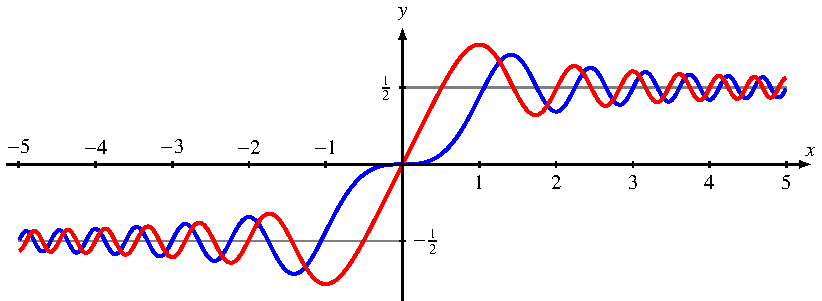
\includegraphics{papers/fresnel/images/fresnelgraph.pdf}
\caption{Graph der Funktionen $C(x)$ ({\color{red}rot}) 
und $S(x)$ ({\color{blue}blau})
\label{fresnel:figure:plot}}
\end{figure}
Die Abbildung~\ref{fresnel:figure:plot} zeigt die Graphen der
Funktion $C(x)$ und $S(x)$.

